\documentclass[11pt,a4paper]{article}
\usepackage[margin=2.0cm,top=1.8cm,bottom=1.8cm]{geometry}
\usepackage[T1]{fontenc}
\usepackage[utf8]{inputenc}
\usepackage{lmodern}
\usepackage{amsmath,amssymb}
\usepackage{siunitx}
\usepackage{booktabs}
\usepackage{graphicx}
\usepackage{caption}
\usepackage{fancyhdr}
\usepackage[hidelinks]{hyperref}
\sisetup{
  separate-uncertainty = true,
  per-mode             = symbol,
  reset-text-series    = false,
  text-series-to-math  = true,
}
\DeclareSIUnit{\angstrom}{\text{\AA}}
\captionsetup{font=small,labelfont=bf,skip=4pt}
\setlength{\textfloatsep}{8pt}\setlength{\intextsep}{8pt}
\setlength{\parskip}{2pt}

% footer required on every page (including the \maketitle page)
\fancypagestyle{plain}{\fancyhf{}\renewcommand{\headrulewidth}{0pt}%
  \cfoot{\small\itshape AI-generated reference solution, not for submission}\rfoot{\small\thepage}}
\pagestyle{plain}

\newcommand{\vb}[1]{\vec{#1}}

\title{\vspace{-1.3cm}MATE70020 Problem Set 2}
\author{Name / CID: [placeholder]}
\date{10 November 2026}

\begin{document}
\maketitle
\vspace{-0.9cm}

\noindent\fbox{\parbox{\dimexpr\linewidth-2\fboxsep-2\fboxrule}{\bfseries
AI NOTICE: This document was generated entirely by an AI agent (Claude Code, Claude Opus 5.5, 10 November 2026) for comparison purposes only. All calculations, figures and text are AI-produced. It is not a student submission and must not be submitted for assessment.}}

\section*{Method}
All calculations used \texttt{pw.x} and \texttt{bands.x} (Quantum ESPRESSO 7.6 [3]) with the supplied LDA
(Perdew--Zunger) pseudopotentials \texttt{B.pz-vbc.UPF} and \texttt{N.pz-vbc.UPF}. The SCF calculation used
\texttt{BN.in} unchanged: \SI{60}{Ry} cutoff, $a=\SI{2.504}{\angstrom}$, $c=\SI{20.0}{\angstrom}$,
$6\times6\times1$ $k$-grid, \texttt{nbnd = 8}. It converged in 7 iterations (estimated accuracy
\SI{3e-7}{Ry}, below the default threshold of \SI{e-6}{Ry}), with $E_\text{tot}=\SI{-25.77488}{Ry}$.
The band structure was then computed non-self-consistently on this density. Only two changes were made to \texttt{BN.in}:
\texttt{calculation = 'bands'}, and \texttt{K\_POINTS crystal\_b} with the path
$\Gamma\,(0,0,0)$~60, $K\,(\tfrac13,\tfrac13,0)$~30, $M\,(\tfrac12,0,0)$~1. This gives 91 $k$-points with
equal spacing \SI{0.028}{\per\angstrom}, because $|\Gamma K|=2|KM|$. The result was post-processed with \texttt{bands.x}.%
\footnote{Inputs, outputs and analysis scripts (folder \texttt{runs/} on branch
\texttt{claude/fervent-ptolemy-sry1eq}): \url{https://github.com/01nietzsch/dfp-ps2}}

\section*{(a) Why the $6\times6\times1$ grid has no $k$-points along $z$}
Quantum ESPRESSO applies periodic boundary conditions in all three directions, so \texttt{BN.in} repeats the
single hBN sheet along $z$ every $c=\SI{20.0}{\angstrom}$ ($\vb a_3=c\,\hat{\vb z}$). Each sheet is separated
from its artificial periodic images by about \SI{20}{\angstrom} of vacuum, like the isolated N$_2$ molecule in a box in
Lecture~3. The Kohn--Sham orbitals of neighbouring sheets do not overlap across this vacuum, so the occupied
KS energies $\varepsilon_{n\vb k}$ do not depend on $k_z$. Every $k_z$ therefore contributes equally to the density
$n(\vb r)=\sum_n\sum_{\vb k}|\psi_{n\vb k}(\vb r)|^2$ (Lecture~4), and the single value $k_z=0$ samples the
zone exactly along $z$. The $k$-grid only has to be converged in the plane of the sheet, where the material is
really periodic. Equivalently, the zone is very thin along $z$: $|\vb b_3|=2\pi/c=\SI{0.314}{\per\angstrom}$,
9.2 times shorter than $|\vb b_1|=\SI{2.897}{\per\angstrom}$ (Table~\ref{tab:recip}). As a check, the occupied
KS energies at $k_z=\pi/c$ (at $\Gamma$ and $K$) differ from those at $k_z=0$ by less than \SI{0.01}{eV}, whereas band~4
disperses by \SI{3.6}{eV} in the plane.

\section*{(b) Primitive lattice vectors and reciprocal lattice vectors}
For \texttt{ibrav = 4} (hexagonal) the INPUT\_PW documentation [1] gives the Cartesian vectors
$\vb a_1=a(1,0,0)$, $\vb a_2=a(-\tfrac12,\tfrac{\sqrt3}{2},0)$ and $\vb a_3=a(0,0,\tfrac ca)$. \texttt{A} and
\texttt{C} are lengths in \si{\angstrom} [1], so with $a=\SI{2.504}{\angstrom}$ and $c=\SI{20.0}{\angstrom}$
\[
  \vb a_1=(2.504,\,0,\,0)~\si{\angstrom},\qquad
  \vb a_2=(-1.252,\,2.169,\,0)~\si{\angstrom},\qquad
  \vb a_3=(0,\,0,\,20.0)~\si{\angstrom}.
\]
The reciprocal vectors follow from $\vb a_i\cdot\vb b_j=2\pi\delta_{ij}$, i.e.\
$\vb b_1=2\pi\,\vb a_2\times\vb a_3/V$ and cyclic permutations, with $V=\vb a_1\cdot(\vb a_2\times\vb a_3)$ (Lecture~4):
\begin{align*}
  \vb a_2\times\vb a_3 &= ac\,(\tfrac{\sqrt3}{2},\tfrac12,0),\quad
  \vb a_3\times\vb a_1 = ac\,(0,1,0),\quad
  \vb a_1\times\vb a_2 = a^2\,(0,0,\tfrac{\sqrt3}{2}),\quad
  V=\tfrac{\sqrt3}{2}a^2c=\SI{108.60}{\angstrom\cubed},\\
  \vb b_1 &= \frac{2\pi}{a}\Big(1,\tfrac{1}{\sqrt3},0\Big),\qquad
  \vb b_2 = \frac{2\pi}{a}\Big(0,\tfrac{2}{\sqrt3},0\Big),\qquad
  \vb b_3 = \frac{2\pi}{c}\,(0,0,1).
\end{align*}
With $2\pi/a=\SI{2.5093}{\per\angstrom}$ and $2\pi/c=\SI{0.31416}{\per\angstrom}$, the numerical values are in
Table~\ref{tab:recip}. $|\vb b_1|=|\vb b_2|=4\pi/(\sqrt3a)=\SI{2.8974}{\per\angstrom}$, and the two vectors are at $60^\circ$
to each other, so the reciprocal lattice is hexagonal. As a check, $\vb a_2\cdot\vb b_1=2\pi(-\tfrac12+\tfrac{\sqrt3}{2}\tfrac{1}{\sqrt3})=0$
and $\vb a_2\cdot\vb b_2=2\pi$; numerically $\vb a_i\cdot\vb b_j=2\pi\delta_{ij}$ to $10^{-15}$. In units of
$2\pi/a$ the vectors are $(1,0.57735,0)$, $(0,1.15470,0)$ and $(0,0,0.12520)$, identical to the reciprocal axes printed by \texttt{pw.x}.

\begin{table}[htb]
\centering
\caption{Primitive reciprocal lattice vectors (b) and high-symmetry points (c): crystal coordinates
(coefficients of $\vb b_1,\vb b_2,\vb b_3$), Cartesian components and length.}
\label{tab:recip}
\small
\begin{tabular}{l c S[table-format=1.4] S[table-format=1.4] S[table-format=1.4] S[table-format=1.4]}
\toprule
 & crystal coord. & {$k_x$ (\si{\per\angstrom})} & {$k_y$ (\si{\per\angstrom})} & {$k_z$ (\si{\per\angstrom})} & {length (\si{\per\angstrom})} \\
\midrule
$\vb b_1$ & $(1,0,0)$ & 2.5093 & 1.4487 & 0      & 2.8974 \\
$\vb b_2$ & $(0,1,0)$ & 0      & 2.8974 & 0      & 2.8974 \\
$\vb b_3$ & $(0,0,1)$ & 0      & 0      & 0.3142 & 0.3142 \\
\midrule
$\Gamma$  & $(0,0,0)$ & 0      & 0      & 0      & 0      \\
$K$       & $(\tfrac13,\tfrac13,0)$ & 0.8364 & 1.4487 & 0 & 1.6728 \\
$M$       & $(\tfrac12,0,0)$ & 1.2546 & 0.7244 & 0 & 1.4487 \\
\bottomrule
\end{tabular}
\end{table}

\section*{(c) $K$ and $M$ in terms of the primitive reciprocal lattice vectors}
The first Brillouin zone is the region closer to $\vb G=0$ than to any other $\vb G$ (Lecture~4). Its boundary is
formed by the perpendicular bisectors of the six shortest $\vb G$, namely $\pm\vb b_1$, $\pm\vb b_2$ and $\pm(\vb b_2-\vb b_1)$, which all have
length $|\vb b_1|$.

\textbf{$M$ (middle of a side).} The side belonging to $\vb b_1$ is its perpendicular bisector, and the midpoint of that side is where it
crosses the line from $\Gamma$ to $\vb b_1$. So $\vb k_M=\tfrac12\vb b_1$, i.e.\ crystal coordinates $(\tfrac12,0,0)$.

\textbf{$K$ (corner).} The sides belonging to $\vb b_1$ and $\vb b_2$ meet at a corner, which is therefore equidistant from $\Gamma$,
$\vb b_1$ and $\vb b_2$. Write $\vb k_K=x\vb b_1+y\vb b_2$ and use $|\vb b_1|^2=|\vb b_2|^2\equiv B^2$ and $\vb b_1\cdot\vb b_2=B^2/2$:
\[
  |\vb k_K|=|\vb k_K-\vb b_1|\Rightarrow 2\vb k_K\cdot\vb b_1=B^2\Rightarrow 2x+y=1,\qquad
  |\vb k_K|=|\vb k_K-\vb b_2|\Rightarrow x+2y=1,
\]
so $x=y=\tfrac13$. Hence $\vb k_K=\tfrac13\vb b_1+\tfrac13\vb b_2$, crystal coordinates $(\tfrac13,\tfrac13,0)$; $\Gamma$ is $(0,0,0)$.

\textbf{Check in Cartesian coordinates.}
$\vb k_K=\tfrac{2\pi}{a}(\tfrac13,\tfrac{1}{\sqrt3},0)$ and $\vb k_M=\tfrac{2\pi}{a}(\tfrac12,\tfrac{1}{2\sqrt3},0)$
(Table~\ref{tab:recip}). These give $|\Gamma K|=4\pi/(3a)=\SI{1.6728}{\per\angstrom}$, $|\Gamma M|=2\pi/(\sqrt3a)=\SI{1.4487}{\per\angstrom}$
and $|KM|=2\pi/(3a)=\SI{0.8364}{\per\angstrom}$. In a regular hexagon the distance to a corner equals the side length $s$, and the
distance to the middle of a side is $\tfrac{\sqrt3}{2}s$. Here $|\Gamma M|/|\Gamma K|=\sqrt3/2$ and $|KM|=\tfrac12|\Gamma K|$, so $M$ is
the midpoint of the side that starts at $K$ and runs to $K'=(\tfrac23,-\tfrac13,0)$, as in the sketch on the problem sheet. A numerical search over $\vb G$
also confirms that $K$ is equidistant from its 3 nearest $\vb G$ (a corner) and $M$ from its 2 nearest (a side midpoint).

\section*{(d) Band structure of monolayer hBN}
The pseudopotentials have $Z_\text{val}=3$ (B) and $5$ (N), so there are 8 valence electrons per cell. In a
spin-unpolarised calculation each band holds 2 electrons, so bands 1--4 are occupied and bands 5--8 are empty
(Fig.~\ref{fig:bands}). The valence-band maximum (top of band~4) and the conduction-band minimum (bottom of band~5)
are both at $K$ (Table~\ref{tab:edges}). \textbf{hBN therefore has a direct band gap at $K$,
$E_g=\varepsilon_{5,K}-\varepsilon_{4,K}=\SI{0.207}{eV}-(\SI{-4.343}{eV})=\SI{4.55}{eV}$.} A path three times denser (271
$k$-points) and a fine path within \SI{0.17}{\per\angstrom} of $K$ (201 $k$-points) give the same location and the same gap.

\begin{figure}[htb]
\centering
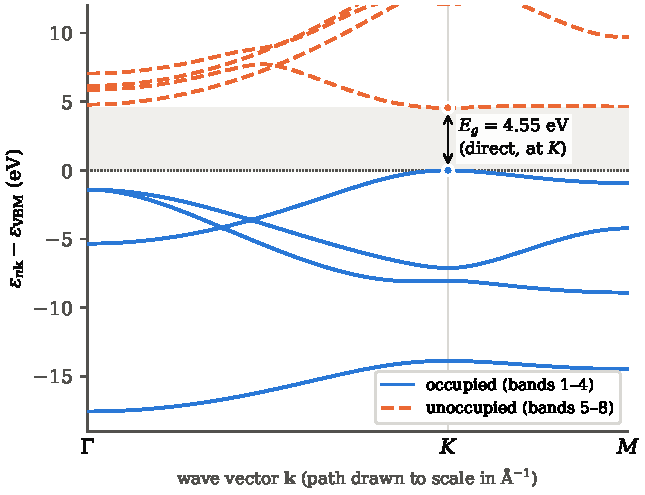
\includegraphics[width=0.6\textwidth]{runs/bands.pdf}
\caption{LDA Kohn--Sham band structure of monolayer hBN along $\Gamma$--$K$--$M$ (path to scale:
$|\Gamma K|=\SI{1.673}{\per\angstrom}$, $|KM|=\SI{0.836}{\per\angstrom}$). Energies are relative to the valence-band maximum.
Solid blue: occupied bands 1--4. Dashed orange: unoccupied bands 5--8. Shading: band gap.}
\label{fig:bands}
\end{figure}

\begin{table}[htb]
\centering
\caption{Valence (band 4) and conduction (band 5) band edges at the high-symmetry points, relative to the VBM.
The band extrema are in bold.}
\label{tab:edges}
\small
\begin{tabular}{l S[table-format=-1.3] S[table-format=1.3] S[table-format=1.3]}
\toprule
 & {band 4 (eV)} & {band 5 (eV)} & {direct gap (eV)} \\
\midrule
$\Gamma$ & -1.398 & 4.793 & 6.191 \\
$K$      & \bfseries 0.000 & \bfseries 4.550 & \bfseries 4.550 \\
$M$      & -0.928 & 4.651 & 5.579 \\
\bottomrule
\end{tabular}
\end{table}

\begin{table}[htb]
\centering
\caption{Band gap of monolayer hBN compared with the experimental value \SI{6.1}{eV} [2].}
\label{tab:compare}
\small
\begin{tabular}{l l l}
\toprule
Method & $E_g$ & error vs.\ \SI{6.1}{eV} \\
\midrule
LDA (\texttt{pz-vbc}, this work) & \SI{4.55}{eV}, direct at $K$ & \SI{-1.55}{eV} ($-25\,\%$) \\
Experiment [2]                   & \SI{6.1}{eV}, direct         & --- \\
\bottomrule
\end{tabular}
\end{table}

\textbf{Comparison with experiment.} The measured gap of monolayer hBN is \SI{6.1}{eV}, and it is also direct [2]. LDA reproduces the
direct character but underestimates the gap by \SI{1.55}{eV} (about 25\,\%, Table~\ref{tab:compare}). This is the known failure discussed in Lecture~3.
LDA and GGAs work well for structural, elastic and vibrational properties but are inaccurate for band gaps of solids, and
semi-local functionals systematically underestimate them. Two reasons apply here. First, the KS energies are eigenvalues of the
fictitious non-interacting system, not true excitation energies (Lecture~2). Second, LDA takes $\epsilon_{xc}$ from the
homogeneous electron gas, evaluated locally. Its approximate exchange does not cancel the spurious interaction of each electron with its own
density, which is contained in the Hartree term; exact (Hartree--Fock) exchange does cancel it. Hybrid functionals such as PBE0 replace 25\,\% of the
semi-local exchange by Hartree--Fock exchange, which opens the gap towards experiment, but they are roughly an order of magnitude more expensive.

\section*{References}
{\small
[1] Quantum ESPRESSO, \emph{Input File Description, Program pw.x} (INPUT\_PW): entries \texttt{ibrav}, \texttt{A}/\texttt{C},
\texttt{K\_POINTS}; \url{https://www.quantum-espresso.org/Doc/INPUT_PW.html} (accessed 10 Nov 2026).\\
{[2]} C.~Elias, P.~Valvin, T.~Pelini, A.~Summerfield, C.~J.~Mellor, T.~S.~Cheng, L.~Eaves, C.~T.~Foxon, P.~H.~Beton, S.~V.~Novikov,
B.~Gil, G.~Cassabois, ``Direct band-gap crossover in epitaxial monolayer boron nitride'', \emph{Nat.\ Commun.} \textbf{10}, 2639 (2019),
doi:10.1038/s41467-019-10610-5.\\
{[3]} P.~Giannozzi \emph{et al.}, \emph{J.\ Phys.: Condens.\ Matter} \textbf{29}, 465901 (2017).\par}

\end{document}
